\section{Tecnologie e strumenti}
\subsection{Git}

Git è un sistema di controllo di versione sviluppato per facilitare la cooperazione nello sviluppo di software. Questo software di versionamento è gratuito ed open-source;  è stato sritto  da \textit{Linus Torvalds} per lo sviluppo del kernel linux nel 2005 ed attualmente mantenuto da \textit{Junio Hamano}. \\
Questo strumento permette di sottomettere al server le modifiche e lasciare ad esso l'onere di verificare se la versione appena inoltrata va in conflitto con quella esistente indicando esattamente in quale punto si è presentato il problema. \\
Viene data la possibilità di generare diversi rami (\textit{branch}) con l'intento di differenziare una nuova versione del codice (\textit{fork}) o per lo sviluppo di una nuova funzionalità, mentre nel primo caso il ramo diverge dal ramo da quale ha origine, nel secondo caso il \textit{branch} ha come fine il ricongiungimento con la sorgente da cui proviene una volta soddisfatto il suo contratto. È proprio da questa idea che nasce il concetto di \texttt{git-flow}.

\subsubsection{\texttt{git-flow}}
\begin{figure}[H]
\begin{center}
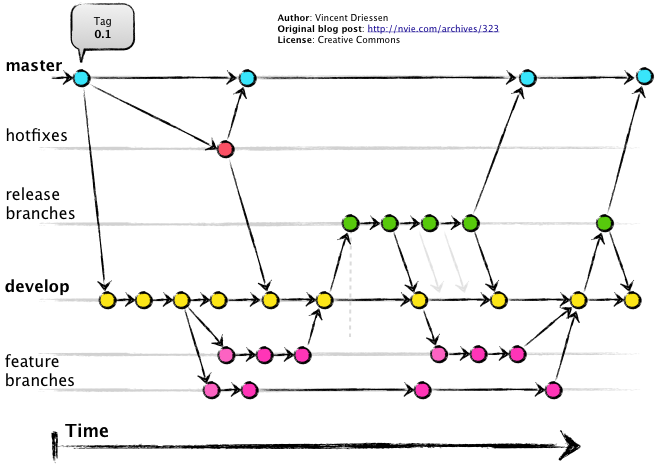
\includegraphics[width=12cm]{Pics/gitflow.png}
\caption{Grafico dei branch di \texttt{git-flow}}
\label{fig:GitFlow}
\end{center}
\end{figure}
Git-flow è un set di estensioni di git che offre dei comandi di alto livello sul repository per utilizzare il modello di branching (vedi \autoref{fig:GitFlow}) di \textit{Vincent Driessen}, fornendo il supporto a branching e release management.
Esso prevede due branch principali:
\begin{itemize}
\item \texttt{"master"}: ramo contenente il codice pronto per essere inoltrato nell'ambiente di produzione;
\item \texttt{"develop"}: ramo di riferimento per l'attività di sviluppo.
\end{itemize}
Sono previste inoltre altre tre tipologie di branch:
\begin{itemize}
\item \texttt{feature}: questo tipo di branch viene creato a partire dal ramo principale \texttt{develop}; dopo aver portato a compimento una particolare funzionalità, il branch \texttt{feature} viene fuso con lo stesso \texttt{develop};
\item \texttt{release}: questo branch è dedicato alla preparazione di un prodotto alla release; qui è possibile effettuare solo piccoli interventi di rimozione di bug (minor bugfix) in vista di un imminente rilascio nel branch master simultaneamente alla pubblicazione della nuova versione con il comando \texttt{git tag};
\item \texttt{hotfix}: questo ramo ha lo scopo di risolvere velocemente eventuali bug riscontrati; ha sempre origine dal branch master e, andando a modificare del software già rilasciato, provoca un avanzamento di sul numero di versione.
\end{itemize}
\paragraph{Vantaggi} 
\begin{itemize}
	\item Permette di mantenere una storia \hl{chiara e concisa} del progetto poiché tutti i commit parziali avvengono nei branch di tipo feature.  Nel ramo develop, saranno presenti solo commit derivanti dalla fusione di rami di tipo feature che soddisfano pienamente il contratto per i quali sono stati creati;
	\item Evita di creare confusione nel repository con commit parziali potenzialmente dannosi e, dualmente, evitare le situazioni in cui lo sviluppo avviene localmente con un solo commit di grosse dimensioni al compimento del contratto del requisito perdendo i vantaggi dello storico dei commit offerti da git.
\end{itemize}
\paragraph{Svantaggi}
\begin{itemize}
	\item L'utilizzo di git-flow richiede agli sviluppatori di dedicare del tempo in più rispetto al metodo classico. Questo però è vero solo per progetti di piccole dimensioni poiché, al crescere dei progetti, il tempo impiegato a risolvere i conflitti derivanti dall'operare in modo classico risulta superiore a quello dedicato ad un corretto utilizzo di git-flow.
	\item Un ulteriore svantaggio è dato dal fatto che gli strumenti offerti dagli IDE per la gestione di git-flow non sono sempre all'altezza del loro compito.
\end{itemize}

\subsection{Rubymine}

\begin{figure}[H]
\begin{center}

\includegraphics[width=4cm]{Pics/rubymine_logo.png}
\caption{Logo di RubyMine}
\label{fig:RubyMine}
\end{center}
\end{figure}
Rubymine è un IDE prodotto da jetBrains, disegnato appositamente per lo sviluppo con Ruby on Rails.
\paragraph{Vantaggi}
\begin{itemize}
	\item Vengono messi a disposizione molti plugin gratuiti che offrono funzionalità specifiche, non incluse nel pacchetto base;
	\item Il salvataggio di un file avviene automaticamente ogni volta che esso perde il focus, dando la garanzia di lavorare sempre con file aggiornati;
	\item Il software è strutturato in modo tale da fornire aiuto attivo nel momento della stesura del codice, come autompletamento ed analisi statica, rendendo più veloce ed efficace il lavoro.
\end{itemize}
\paragraph{Svantaggi}
\begin{itemize}
	\item Il plugin responsabile del versionamento non funziona sempre alla perfezione, in particolare quando si utilizza git-flow.
\end{itemize}

\subsection{Ruby on Rails}

Ruby on Rails, è un framework open source per lo sviluppo di applicazioni web.
La sua architettura si basa sul pattern Model-View-Controller (MVC), realizzando a tutti gli effetti un framework full-stack; è dunque possibile realizzare sia la parte di backend che quella di frontend.
\paragraph{Vantaggi}
\begin{itemize}
	\item Risorse e componenti sono integrati in modo tale che i collegamenti non debbano mai essere impostati manualmente, ma in modo automatico;
	\item È possibile lavorare utilizzando ActiveRecord, descritto nella sezione \ref{sec:ActiveRecord}. Questo è un grosso vantaggio perché velocizza la stesura del codice e risponde bene ai cambiamenti. Nel progetto svolto \hl{, l'utilizzo di ActiveRecord} è un fattore determinante poiché è necessario che il software sia sempre conforme alle normative vigenti che cambiano nel tempo;
	\item \hl{È possibile disaccoppiare il backend ed il frontend} perché in rails il routing delle risorse è gestito con una interfaccia REST;
	\item Sono inoltre messi a disposizione i seguenti ambienti per uno stesso software, al fine di creare una separazione nel progetto:
		\begin{itemize}
		\item development 
		\item test
		\item production
		\end{itemize} 
		Ambienti distinti solitamente risiedono anche su server distinti.
	\item Sono presenti infine numerose librerie dette \textit{Gemme}, che offrono molteplici funzionalità velocizzando il lavoro.
\end{itemize}
\paragraph{Svantaggi}
	\begin{itemize}
		\item Ruby on rails è meno performante rispetto ad altri linguaggi, ad esempio Java o Scala, ma di un ordine di grandezza non influente su progetti di medie dimensioni. 
	\end{itemize} 
		
\subsubsection{ActiveRecord}

\label{sec:ActiveRecord}
Active Record è il modulo di Ruby on Rails che gestisce la persistenza dei dati seguendo il pattern Active-Record di Martin Fowler 
%\citep{MartinFowler:patterns}
, il quale si serve di un database.
Esso prevede:
\begin{itemize}
\item Ogni tabella del database relazionale è gestita attraverso una classe;
\item Una singola istanza della classe corrisponde ad una riga (record) nella tabella associata;
\item Alla creazione di una nuova istanza viene creata una nuova riga all'interno della tabella che viene aggiornata ad ogni modifica dell'istanza associata.
\end{itemize}
Le colonne della tabella sono rappresentate come attributi della classe.

\paragraph{Vantaggi} 
\begin{itemize}
	\item È possibile associare un diverso database per ogni ambiente predisposto da Rails separando i record memorizzati per lo sviluppo, per i test, o per l'ambiente di produzione;
	\item È disponibile un meccanismo di gestione delle relazioni molto efficiente che facilita dichiarazione ed utilizzo delle diverse tipologie di relazione tra le tabelle del database;
	\item Viene messo a disposizione un meccanismo specifico per la gestione dell'evoluzione dello schema del database mediante le \texttt{migrazioni} (vedi \autoref{App:AppendiceMigrazioni}). 
\end{itemize} 
\paragraph{Svantaggi}
\begin{itemize}
	\item Richiede una progettazione spesso diversa da quella classica, poiché l'ereditarietà risulta molto più difficile da gestire quando una classe corrisponde ad una tabella;
	\item Ad ogni migrazione, è necessario pensare bene a tutti gli effetti collaterali che potrebbero avvenire sugli statement che utilizzano la tabella modificata.
\end{itemize} 

\subsubsection{ActiveAdmin}

\begin{figure}[H]
\begin{center}

\includegraphics[width=6cm]{Pics/ActiveAdmin_logo.png}
\caption{Logo di ActiveAdmin}
\label{fig:ActiveAdminLogo}
\end{center}
\end{figure}
ActiveAdmin è una libreria (Gemma) di Ruby on Rails che permette di creare un sistema di amministrazione (backoffice). Mediante un pannello di gestione, permette di inserire, eliminare ed aggiornare istanze di modelli e relazioni direttamente da browser. 
\paragraph{Vantaggi}
\begin{itemize}
	\item Questa libreria permette ad un utente del sito di essere autonomo nell'aggiornamento dei contenuti senza dover attendere i tempi tecnici dell'azienda fornitrice;
	\item È fortemente personalizzabile, per questo è spesso utilizzato per la creazione di Dashboard o altre funzionalità dedicate ad utenti ai quali sono assegnati particolari privilegi d'accesso.
\end{itemize}
\paragraph{Svantaggi}
\begin{itemize}
	\item La grafica di ActiveAdmin risulta datata, è quindi spesso necessario riprogettare la veste grafica del pannello di amministrazione fornito di default.
\end{itemize}
\subsubsection{I18n}
	\hl{ NUOVA SEZIONE}
	\begin{figure}[H]
		\begin{center}
			
\includegraphics[width=4cm]{Pics/i8n-logo.png}
			\caption{Logo di I18n}
			\label{fig:I18NLogo}
		\end{center}
	\end{figure}
	I18n è l'abbreviazione della parola "internationalization", deriva dal suo spelling che interpone 18 lettere tra la "i" iniziale e la "n" finale. \\ 
	Lo scopo è gestire la distribuzione del software in diverse lingue. Il meccanismo prevede un codice identificativo per ogni stringa da visualizzare, che assumerà un diverso valore per ogni traduzione. \\
	In Ruby, esiste una apposita gemma, denominata appunto \textit{I18N}, che fornisce le direttive per adottare correttamente questo approccio. \\
	Spesso il concetto di internazionalizzazione, viene associato a quello di localizzazione che è l'insieme dei processi di adattamento di un software , pensato e progettato per un mercato e contesto predefinito, in modo specifico ad altre nazione e culture. \\
	Tutte le informazioni di pertinenza di una lingua sono raccolti in un gruppo di parametri chiamato \textit{locale}.
\paragraph{Vantaggi}
	\begin{itemize}
		\item Grazie alla gemma \textit{i18n} , è possibile riutilizzare il codice responsabile della logica di business dell'applicazione e localizzare le stringhe per ogni lingua;
		\item L'aggiunta di nuove lingue richiede solo lo sforzo riguardante la traduzione ed eventuali conversioni nelle unità di misura appropriate;
		\item È possibile riutilizzare in contesti diversi le stringhe già definite, evitando quindi di introdurre errori di battitura;
		\item L'aggiunta di nuove lingue non provoca alcuna modifica nell'applicazione esistente, ma solo l'aggiunta del file in formato \texttt{yml} con le traduzioni.
	\end{itemize}
\paragraph{Svantaggi}
	\begin{itemize}
		\item La scrittura di codice con questo approccio richiede generalmente più tempo se il software esiste in una sola lingua.
	\end{itemize}
\subsection{JRuby}
	\hl{NUOVA SEZIONE}
	\begin{figure}[H]
		\begin{center}
			
\includegraphics[width=4cm]{Pics/jruby-logo.png}
			\caption{Logo di JRuby}
			\label{fig:JRubyLogo}
		\end{center}
	\end{figure}
	JRuby è un'implementazione in Java del linguaggio di programmazione Ruby. \\
	Sebbene non siano coperte tutte le implementazioni delle librerie standard offerte da Ruby, è comunque possibile utilizzare tutti la maggior parte delle funzionalità del  linguaggio.
\paragraph{Vantaggi}
\begin{itemize}
	\item JRuby è un software completamente gratuito;
	\item Gira su una JVM, quindi è possibile integrare l'interprete Ruby in una applicazione Java ed, allo stesso tempo, scrivere direttamente codice Java.
\end{itemize}
\paragraph{Svantaggi}
	\begin{itemize}
		\item È possibile incontrare situazioni in cui si necessita di una libreria che non è stata implementata;
		\item L'utilizzo di JRuby provoca un significativo appesantimento del software ed un conseguente peggioramento delle performance. 
	\end{itemize}
\subsection{Drools}
	\hl{NUOVA SEZIONE}
	\begin{figure}[H]
		\begin{center}
			
\includegraphics[width=7cm]{Pics/drools-logo.png}
			\caption{Logo di Drools}
			\label{fig:DroolsLogo}
		\end{center}
	\end{figure}
	
	
\paragraph{Vantaggi}
\paragraph{Svantaggi}
\subsection{Java}
\paragraph{Vantaggi}
\paragraph{Svantaggi}
\subsection{Foundation}
\paragraph{Vantaggi}
\paragraph{Svantaggi}
\subsection{jQuery}
\paragraph{Vantaggi}
\paragraph{Svantaggi}
\subsection{selectize.js}
\paragraph{Vantaggi}
\paragraph{Svantaggi}